\documentclass[11pt,a4paper]{article}
\usepackage[utf8]{inputenc}
\usepackage[T1]{fontenc}
\usepackage{amsmath,amssymb}
\usepackage{booktabs}
\usepackage{siunitx}
\usepackage{graphicx}
\usepackage{tikz}
\usetikzlibrary{arrows.meta,positioning}
\usepackage[margin=2cm]{geometry}
\usepackage{hyperref}
\sisetup{exponent-product=\times}
\emergencystretch=2em
\begin{document}

\noindent{\Large\bfseries Number of $\nu_e$ appearance events}
\vspace{1ex}\hrule\vspace{2ex}

\begin{equation*}
  N = P(\nu_\mu\to\nu_e; E_0, L)\, \sigma_{CC}(E_0)\, \Phi\, \mathrm{POT}\, N_T
  \;\simeq\; 60.2\,P
  \Big[\tfrac{\sigma_{CC}}{10^{-38}\,\mathrm{cm^2}}\Big]
  \Big[\tfrac{\Phi}{10^{-14}\,\mathrm{cm^{-2}\,POT^{-1}}}\Big]
  \Big[\tfrac{\mathrm{POT}}{10^{21}}\Big]
  \Big[\tfrac{M}{\mathrm{kt}}\Big]
\end{equation*}
The second form follows from writing $N_T = M\,N_A$ (one nucleon per atomic mass unit, $N_A = \SI{6.022e23}{g^{-1}}$)
and measuring each factor in the units in brackets: the constant is
$10^{-38}\cdot10^{-14}\cdot10^{21}\cdot(10^{9}\,\mathrm{g/kt}\cdot\SI{6.022e23}{g^{-1}}) = 60.2$, and all units cancel.
$N$ is the number of $\nu_e$ ($\bar\nu_e$) charged-current interactions in the fiducial volume, i.e., the number of
events seen by a perfect detector (efficiency $=1$). The last section (\emph{Why the experiments see a different number})
explains why the experiments see a different number.

\begin{figure}[!htb]
  \centering
  \resizebox{\textwidth}{!}{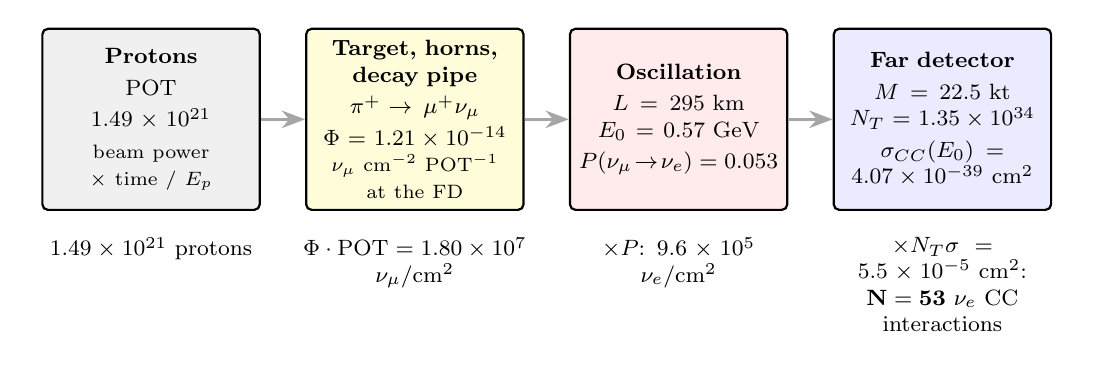
\begin{tikzpicture}[
  font=\footnotesize, >=Stealth,
  blk/.style={draw, rounded corners=2pt, thick, minimum height=2.3cm, text width=2.55cm, align=center, inner sep=3pt},
  lab/.style={font=\footnotesize\bfseries, align=center},
  num/.style={font=\footnotesize, align=center, text width=2.9cm},
  arr/.style={->, very thick, color=gray!70}]
  % blocks
  \node[blk, fill=gray!12]   (p)  at (0,0)    {\textbf{Protons}\\[2pt] $\mathrm{POT}$\\[2pt] $1.49\times10^{21}$\\[2pt]{\scriptsize beam power $\times$ time / $E_p$}};
  \node[blk, fill=yellow!15] (b)  at (3.35,0) {\textbf{Target, horns,\\ decay pipe}\\[2pt] $\pi^+\!\to\mu^+\nu_\mu$\\[2pt] $\Phi = 1.21\times10^{-14}$\\{\scriptsize $\nu_\mu$ cm$^{-2}$ POT$^{-1}$ at the FD}};
  \node[blk, fill=red!8]     (o)  at (6.7,0)  {\textbf{Oscillation}\\[2pt] $L = 295$ km\\ $E_0 = 0.57$ GeV\\[2pt] $P(\nu_\mu\!\to\!\nu_e) = 0.053$};
  \node[blk, fill=blue!8]    (d)  at (10.05,0){\textbf{Far detector}\\[2pt] $M = 22.5$ kt\\ $N_T = 1.35\times10^{34}$\\[2pt] $\sigma_{CC}(E_0) = 4.07\times10^{-39}$ cm$^2$};
  \foreach \a/\b in {p/b, b/o, o/d} \draw[arr] (\a.east) -- (\b.west);
  % running result under each block
  \node[num, below=6pt of p] {$1.49\times10^{21}$ protons};
  \node[num, below=6pt of b] {$\Phi\cdot\mathrm{POT} = 1.80\times10^{7}$\\ $\nu_\mu$/cm$^2$};
  \node[num, below=6pt of o] {$\times P$: $9.6\times10^{5}$\\ $\nu_e$/cm$^2$};
  \node[num, below=6pt of d] {$\times N_T\sigma = 5.5\times10^{-5}$ cm$^2$:\\ $\mathbf{N = 53}$ $\nu_e$ CC interactions};
\end{tikzpicture}
}
  \caption{The chain of the calculation for the T2K neutrino beam (NuFIT~6.0, normal ordering). Each block is one factor
  of the formula; below each block, the running result. Protons on target produce, through the target, the focusing
  horns and the decay pipe, a $\nu_\mu$ beam: at the far detector it gives $\Phi$ neutrinos per cm$^2$ per POT. A fraction
  $P$ oscillates into $\nu_e$ over the baseline $L$; the far detector offers a target area $N_T\,\sigma_{CC}$.}
  \label{fig:scheme}
\end{figure}

\begin{itemize}
  \item $\Phi\times\mathrm{POT}$ is the \textbf{beam side}: the number of $\nu_\mu$ crossing each cm$^2$ of the far
        detector (how the beam is produced: Fig.~\ref{fig:beamline}). $\Phi = \int (d\Phi/dE)\,dE = \sum_k (d\Phi/dE)_k\,\Delta E_k$ is the $\nu_\mu$ ($\bar\nu_\mu$) flux per proton on target \emph{integrated over the whole energy spectrum} (not taken at $E_0$), summing the bins of the public flux histograms
        (T2K: Phys.\ Rev.\ D 87, 012001 (2013); NOvA: FERMILAB-DATA-2017-01; DUNE: arXiv:2103.04797), see Fig.~\ref{fig:flux}.
        POT is the exposure, $\mathrm{POT} = \text{beam power}\times\text{time}/\text{proton energy}$.
  \item $\sigma_{CC}\times N_T$ is the \textbf{detector side}: the target area seen by a neutrino.
        $N_T = M N_A$ is the number of nucleons in the fiducial mass $M$; $\sigma_{CC}$ is the inclusive
        charged-current cross section per nucleon (GLoBES tables, Comput.\ Phys.\ Commun.\ 167, 195 (2005);
        GENIE on argon for DUNE, arXiv:2103.04797), see Fig.~\ref{fig:xsec}.
  \item $P$ is the oscillation probability in matter (NuFast, arXiv:2405.02400), here at the NuFIT~6.0 best fit
        (JHEP 12 (2024) 216). It is the only factor that depends on the oscillation parameters: varying $\delta_{CP}$,
        the mass ordering or $\theta_{23}$ changes $N$ only through $P$, all other factors fixed.
  \item $E_0$ replaces the energy spectrum by a single energy, the mean energy of the beam peak.
  \item \textbf{Assumptions}: pure $\nu_\mu$ ($\bar\nu_\mu$) beam, one energy, every interaction detected,
        no backgrounds, constant matter density. The formula gives no energy spectrum.
%   \item \textbf{Sensitivity}: each sample has a statistical error $\sqrt N$; comparing the true $\delta_{CP}$ with the
%         CP-conserving values,
%         $\Delta\chi^2 = \min_{\delta'\in\{0,\pi\}} \sum_{\nu,\bar\nu} [N(\delta_{CP})-N(\delta')]^2/N(\delta_{CP})$,
%         with significance $\sqrt{\Delta\chi^2}$ (PDG, Statistics review).
\end{itemize}

\begin{figure}[!htb]
  \centering
  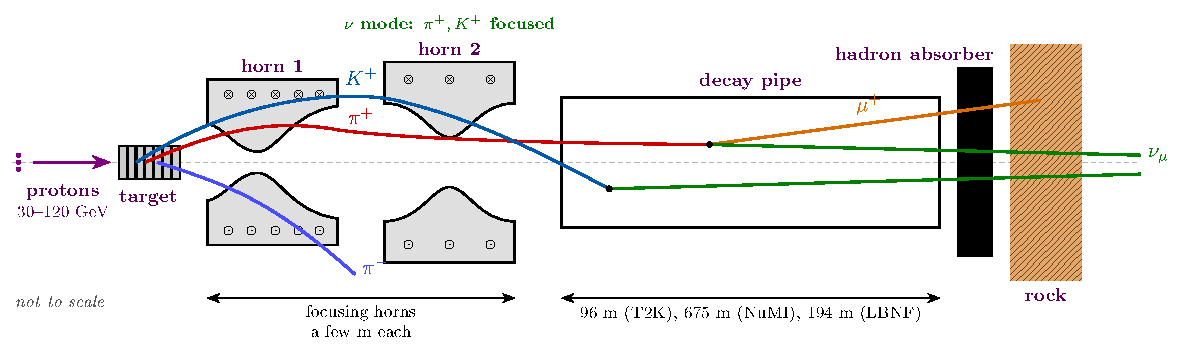
\includegraphics[width=\textwidth]{figures/beamline.pdf}
  \caption{Schematic of an accelerator neutrino beam in neutrino mode (not to scale). Protons hit a graphite target and
  produce mesons. Two magnetic horns, with a toroidal field between the inner and outer conductors, focus the
  positive mesons ($\pi^+$, $K^+$) towards the beam axis and defocus the negative ones ($\pi^-$). The mesons decay in
  the decay pipe, mainly $\pi^+\to\mu^+\nu_\mu$; the absorber and the rock stop the remaining hadrons and the muons,
  and only the neutrinos continue to the detectors. Reversing the horn current focuses $\pi^-$, $K^-$ and gives the
  $\bar\nu_\mu$ beam. Decay pipe lengths: 96~m at T2K, 675~m at NuMI (NOvA), 194~m at LBNF (DUNE).}
  \label{fig:beamline}
\end{figure}

\noindent\begin{minipage}{\textwidth}
\paragraph{Inputs} (NuFIT~6.0 normal ordering for $P$).

\begin{center}
\footnotesize
\setlength{\tabcolsep}{4pt}
\begin{tabular}{llcccccc}
\toprule
 & beam & $L$ [km] & $M$ [kt] & POT & $E_0$ [GeV] & $\Phi$ [$10^{-14}$/cm$^2$/POT] & $\sigma_{CC}$ [$10^{-38}$ cm$^2$] \\
\midrule
T2K     & $\nu$     & 295  & 22.5 & \num{1.494e21} & 0.57 & 1.207 & 0.407 \\
        & $\bar\nu$ &      &      & \num{1.635e21} & 0.55 & 0.976 & 0.116 \\
Hyper-K & $\nu$     & 295  & 187  & \num{6.75e21}  & 0.57 & 1.207 & 0.407 \\
        & $\bar\nu$ &      &      & \num{2.025e22} & 0.55 & 0.976 & 0.116 \\
NOvA    & $\nu$     & 810  & 14   & \num{2.661e21} & 1.80 & 1.806 & 1.43 \\
        & $\bar\nu$ &      &      & \num{1.25e21}  & 1.79 & 1.467 & 0.631 \\
DUNE    & $\nu$     & 1300 & 40   & \num{7.15e21}  & 2.31 & 1.548 & 1.78 \\
        & $\bar\nu$ &      &      & \num{7.15e21}  & 2.27 & 1.385 & 0.729 \\
\bottomrule
\end{tabular}
\end{center}
\end{minipage}

\bigskip

\noindent\begin{minipage}{\textwidth}
\paragraph{Worked out} ($N_{P=1} = 60.2\,\sigma\,\Phi\,\mathrm{POT}\,M$ in the units above, then $\times P$).

\begin{center}
\small
\begin{tabular}{llcc}
\toprule
 & beam & $N_{P=1}$ & $N = N_{P=1}\times P$ \\
\midrule
T2K     & $\nu$     & $60.2\times0.407\times1.207\times1.494\times22.5 = 994$     & $\times0.0533=\mathbf{53}$ \\
        & $\bar\nu$ & $60.2\times0.116\times0.976\times1.635\times22.5 = 251$     & $\times0.0316=\mathbf{7.9}$ \\
Hyper-K & $\nu$     & $60.2\times0.407\times1.207\times6.75\times187 = 37\,329$   & $\times0.0533=\mathbf{1990}$ \\
        & $\bar\nu$ & $60.2\times0.116\times0.976\times20.25\times187 = 25\,809$  & $\times0.0316=\mathbf{816}$ \\
NOvA    & $\nu$     & $60.2\times1.43\times1.806\times2.661\times14 = 5792$       & $\times0.0547=\mathbf{317}$ \\
        & $\bar\nu$ & $60.2\times0.631\times1.467\times1.25\times14 = 975$        & $\times0.0249=\mathbf{24}$ \\
DUNE    & $\nu$     & $60.2\times1.78\times1.548\times7.15\times40 = 47\,441$     & $\times0.0738=\mathbf{3501}$ \\
        & $\bar\nu$ & $60.2\times0.729\times1.385\times7.15\times40 = 17\,384$    & $\times0.0178=\mathbf{309}$ \\
\bottomrule
\end{tabular}
\end{center}
\end{minipage}

\paragraph{Sensitivity to CP violation.}
Each experiment measures two numbers, $N_\nu$ and $N_{\bar\nu}$. The agreement between observed numbers
$N_i^\text{obs}$ and the prediction $N_i^\text{pred}$ of a hypothesis is measured with
\begin{equation*}
  \chi^2 = \sum_{i=\nu,\bar\nu} \frac{\left(N_i^\text{obs} - N_i^\text{pred}\right)^2}{\sigma_i^2},
  \qquad \sigma_i^2 = N_i^\text{obs},
\end{equation*}
since the number of events is Poisson distributed and its statistical variance equals the number of events
(no normalization uncertainty is included). For the expected sensitivity:
(i) the observed numbers are the prediction for the true value, $N_i^\text{obs} = N_i(\delta_{CP})$, without
fluctuations, so the best fit is the true value itself, with $\chi^2 = 0$;
(ii) CP conservation means $\delta_{CP} = 0$ or $\pi$: both must be rejected, so we keep the one that fits best;
(iii) $\Delta\chi^2$, the difference from the best fit ($\chi^2=0$), is then
\begin{equation*}
  \boxed{\;\Delta\chi^2(\delta_{CP}) = \min_{\delta'\in\{0,\pi\}} \sum_{i=\nu,\bar\nu}
  \frac{\left[N_i(\delta_{CP}) - N_i(\delta')\right]^2}{N_i(\delta_{CP})},
  \qquad \text{significance} = \sqrt{\Delta\chi^2}\ \sigma\;}
\end{equation*}
with $N_i$ from the formula above (only $P$ changes with $\delta_{CP}$). For one parameter, $\Delta\chi^2 = 9$ ($25$)
corresponds to $3\sigma$ ($5\sigma$) (PDG, Review of Particle Physics, Statistics chapter).
The CP-violation sensitivity is defined, as in the DUNE (arXiv:2002.03005) and Hyper-K (arXiv:1805.04163) design studies,
as $\sqrt{\Delta\chi^2}$ with respect to $\delta_{CP} = 0, \pi$ computed on Asimov data. Our version is a simplified
counting version: Gaussian statistics, two samples, no backgrounds, fixed oscillation parameters.
With the numbers of the table (true normal ordering, statistical errors only), the maximum significance over
$\delta_{CP}$ is $2.5\sigma$ (T2K), $4.4\sigma$ (NOvA), $17\sigma$ (Hyper-K) and $18\sigma$ (DUNE).
Derivation and the case with a normalization uncertainty: \texttt{docs/number\_of\_events.pdf}.

\section*{Why the experiments see a different number}
\label{sec:r}

The collaborations publish the number of appearance signal events expected in their analyses, computed with full
simulations of beam, cross sections and detector. Evaluating our formula with the same oscillation parameters, the
ratio
\begin{equation*}
  r = \frac{N_\text{published}}{N}
\end{equation*}
would be 1 if the formula were exact. Table~\ref{tab:r} shows that it is not: $r = 0.4$--$1.1$.
Writing the published number as an integral over the spectrum, $r$ splits into two factors,
\begin{equation*}
  r = \underbrace{\frac{N_\text{published}}{\mathrm{POT}\,N_T\int\Phi(E)\,\sigma(E)\,P(E)\,dE}}_{\varepsilon_\text{det}}
  \times
  \underbrace{\frac{\int\Phi(E)\,\sigma(E)\,P(E)\,dE}{\Phi\,\sigma(E_0)\,P(E_0)}}_{c_\text{mono}} ,
\end{equation*}
which correspond to the two simplifications of the formula:
\begin{itemize}
  \item \textbf{Detection} ($\varepsilon_\text{det}$): not every $\nu_e$ interaction is selected (detector
        efficiency and analysis cuts), so $\varepsilon_\text{det}<1$. In practice $\varepsilon_\text{det}$ also
        absorbs the differences between our cross sections and the generators used by the collaborations.
  \item \textbf{One energy} ($c_\text{mono}$): the beam is not monochromatic. In the $\nu$ beams $E_0$ is close to
        the oscillation maximum, while many neutrinos have energies where $P$ is smaller: the formula overestimates
        the rate, $c_\text{mono}\approx0.8$. In the $\bar\nu$ beams the antineutrino cross section grows quickly with
        energy, so the high-energy part of the flux weighs more: $c_\text{mono}\approx1$ at T2K/Hyper-K and $1.4$ at DUNE.
\end{itemize}
So $r<1$ in the $\nu$ beams, where both effects reduce the rate, and $r\approx1$ or even $>1$ in the $\bar\nu$ beams of
Hyper-K and DUNE, where the one-energy underestimate compensates the efficiency. $r$ is therefore not an efficiency:
it collects everything the formula leaves out. (It is not due to the beam contamination: the references are right-sign
signal only.)

\begin{table}[!htb]
\centering
\caption{Comparison with the published predictions, at the oscillation parameters of each reference.
T2K: Table~XI total single-ring $e$-like events at $\delta_{CP}=-\pi/2$ minus the $\delta_{CP}$-independent background
obtained by fitting the four $\delta_{CP}$ values of the table.}
\label{tab:r}
\footnotesize
\setlength{\tabcolsep}{4pt}
\begin{tabular}{llrrcccl}
\toprule
 & beam & $N$ (formula) & $N_\text{published}$ & $r$ & $c_\text{mono}$ & $\varepsilon_\text{det}=r/c_\text{mono}$ & reference \\
\midrule
T2K     & $\nu$     & 61.6   & 54.8 & 0.89 & 0.81 & 1.10 & arXiv:2101.03779, Table XI \\
        & $\bar\nu$ & 6.7    & 4.8  & 0.71 & 1.06 & 0.68 & arXiv:2101.03779, Table XI \\
Hyper-K & $\nu$     & 2064   & 1643 & 0.80 & 0.85 & 0.94 & arXiv:1805.04163, Tables XXXVI--XXXVII \\
        & $\bar\nu$ & 1156   & 1183 & 1.02 & 1.00 & 1.02 & arXiv:1805.04163, Tables XXXVI--XXXVII \\
NOvA    & $\nu$     & 290.5  & 125.3 & 0.43 & 0.79 & 0.54 & arXiv:2509.04361, Table 2 \\
        & $\bar\nu$ & 37.2   & 18.9 & 0.51 & 0.83 & 0.61 & arXiv:2509.04361, Table 2 \\
DUNE    & $\nu$     & 3486   & 2180 & 0.63 & 0.78 & 0.79 & arXiv:2103.04797, GLoBES configuration \\
        & $\bar\nu$ & 409    & 438  & 1.07 & 1.39 & 0.77 & arXiv:2103.04797, GLoBES configuration \\
\bottomrule
\end{tabular}
\end{table}

\paragraph{Consequences.} Everything that depends only on $P$ (bi-probability plots, shape of the $\delta_{CP}$
dependence, degeneracies) is unchanged. The numbers of events of the formula are those of a perfect detector: about
twice the published ones for NOvA, within ${\sim}40\,\%$ for the other experiments. The significances are optimistic:
multiplying each sample by its $r$, the maximum sensitivity to CP violation (statistics only, true normal ordering)
becomes $2.3\sigma$ (T2K), $2.9\sigma$ (NOvA), $16\sigma$ (Hyper-K) and $16\sigma$ (DUNE). With a $5\,\%$ normalization
uncertainty the Hyper-K and DUNE values ($8.6$--$9.4\sigma$) hardly change, because they are limited by the systematic
uncertainty and not by the number of events.

\newpage

\begin{figure}[!htb]
  \centering
  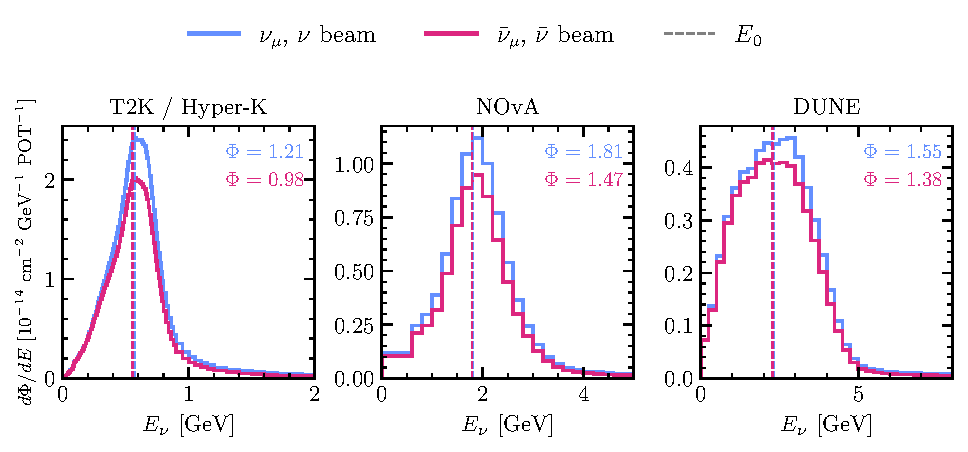
\includegraphics{figures/fluxes.pdf}
  \caption{Unoscillated $\nu_\mu$ flux in the neutrino beam and $\bar\nu_\mu$ flux in the antineutrino beam at the far
  detectors, per proton on target, from the public flux releases (T2K: 2020 release at Super-Kamiokande, also used for
  Hyper-K; NOvA: 2017 near-detector flux $\times\,(1\,\mathrm{km}/810\,\mathrm{km})^2$; DUNE: TDR far-detector flux).
  Dashed lines: the beam energy $E_0$ (flux-weighted mean energy of the main peak). The numbers give
  $\Phi = \sum_k (d\Phi/dE)_k\,\Delta E_k$ in units of $10^{-14}$ cm$^{-2}$ POT$^{-1}$, as used in the table.}
  \label{fig:flux}
\end{figure}

\begin{figure}[!htb]
  \centering
  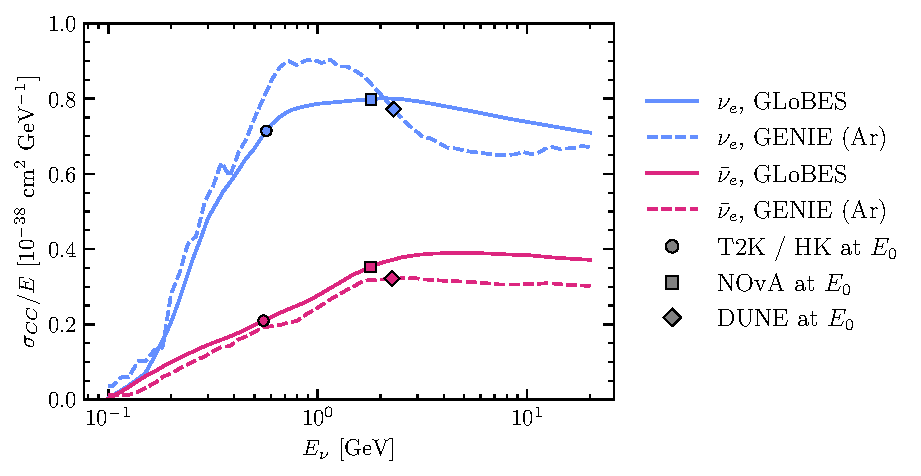
\includegraphics{figures/cross_sections.pdf}
  \caption{Inclusive charged-current cross section per nucleon, divided by energy, for $\nu_e$ and $\bar\nu_e$:
  GLoBES standard table (low energy: Super-Kamiokande cross sections for water, M.~D.~Messier, PhD thesis (1999);
  high energy: Paschos and Yu, Phys.\ Rev.\ D 65, 033002 (2002)), used for T2K, Hyper-K and NOvA; GENIE on argon
  of the DUNE TDR configuration (arXiv:2103.04797), used for DUNE. Markers: $\sigma_{CC}(E_0)/E_0$ entering the table.}
  \label{fig:xsec}
\end{figure}

\end{document}
